\documentclass[12pt,titlepage]{article}
\usepackage[margin=1.25in]{geometry}
\usepackage{graphicx,amsmath,minted}

%% Variables definition
\newcommand{\vSubject}{Matematika 3}
\newcommand{\vSubtitle}{Statistics}
\newcommand{\vName}{Dicha Zelianivan Arkana}
\newcommand{\vNIM}{2241720002}
\newcommand{\vClass}{2i}
\newcommand{\vDepartment}{Information Technology}
\newcommand{\vStudyProgram}{D4 Informatics Engineering}

%% [START] Tikz related stuff
\usepackage{tikz}
\usetikzlibrary{svg.path,calc,shapes.geometric,shapes.misc}
\tikzstyle{terminator} = [rectangle, draw, text centered, rounded corners = 1em, minimum height=2em]
\tikzstyle{preparation} = [chamfered rectangle, chamfered rectangle sep=0.75em, draw, text centered, minimum height = 2em]
\tikzstyle{process} = [rectangle, draw, text centered, minimum height=2em]
\tikzstyle{decision} = [diamond, aspect=2, draw, text centered, minimum height=2em]
\tikzstyle{data}=[trapezium, draw, text centered, trapezium left angle=60, trapezium right angle=120, minimum height=2em]
\tikzstyle{connector} = [line width=0.25mm,->]
%% [END] Tikz related stuff

%% [START] Fancy header related stuff
\usepackage{fancyhdr}
\pagestyle{fancy}
\setlength{\headheight}{15pt} % compensate fancyhdr style
\fancyhead{}
\fancyfoot{}
\fancyfoot[L]{\thepage}
\fancyfoot[R]{\textit{\vSubject - \vSubtitle}}
\renewcommand{\footrulewidth}{0.4pt}% default is 0pt, overline for footer
%% [END] Fancy header related stuff

%% [START] Custom tabular command related stuff
\usepackage{tabularx}
\newcommand{\details}[2]{
    #1 & #2  \\
}
%% [END] Custom tabular command related stuff

%% [START] Figure related stuff
\newcommand{\image}[3][1]{
    \begin{figure}[h]
        \centering
        \includegraphics[#1]{#2}
        \caption{#3}
        \label{#3}
    \end{figure}
}
%% [END] Figure related stuff

\begin{document}
\begin{titlepage}
    \centering
    \vfill
    {\bfseries\LARGE
        \vSubject\\
        \vskip0.25cm
        \vSubtitle
    }
    \vfill
    
\includegraphics[width=6cm]{images/polinema-logo.png}
    \vfill
    {
        \textbf{Name}\\
        \vName\\
        \vskip0.5cm
        \textbf{NIM}\\
        \vNIM\\
        \vskip0.5cm
        \textbf{Class}\\
        \vClass\\
        \vskip0.5cm
        \textbf{Department}\\
        \vDepartment\\
        \vskip0.5cm
        \textbf{Study Program}\\
        \vStudyProgram
    }
\end{titlepage}

\tableofcontents

\pagebreak

\section{Formula}
\subsection{Mean}
\begin{align*}
    \bar{x} &= \frac{\sum_ x}{n}
\end{align*}
Where:
\begin{itemize}
    \item $\bar{x}$ = mean
    \item $\sum_ x$ = sum of all values
    \item $n$ = number of values
\end{itemize}

\subsection{Median}
\subsubsection{Median}
\begin{align*}
    \text{Me} &= \frac{^x(\frac{n}{2})~+~^x(\frac{n}{2}+1)}{2}
\end{align*}
Where:
\begin{itemize}
    \item $\text{Me}$ = median
    \item $^x(\frac{n}{2})$ = value of $\frac{n}{2}$th item
    \item $^x(\frac{n}{2}+1)$ = value of $\frac{n}{2}+1$th item
\end{itemize}

\subsubsection{Grouped Median}
\begin{align*}
    \text{Me} &= b + p \left( \frac{\frac{1}{2}n - F}{f} \right)
\end{align*}
Where:
\begin{itemize}
    \item $\text{Me}$ = median
    \item $b$ = lower boundary of median class
    \item $p$ = class interval
    \item $n$ = number of values
    \item $F$ = cumulative frequency of class before median class
    \item $f$ = frequency of median class
\end{itemize}

\subsection{Mode}
\begin{align*}
    \text{Mode} &= \text{L} + \text{c} \left( \frac{l}{l+u} \right)
\end{align*}
Where:
\begin{itemize}
    \item $\text{Mode}$ = mode
    \item $\text{L}$ = lower boundary of modal class
    \item $\text{c}$ = class interval
    \item $l$ = frequency of modal class and the one before it
    \item $u$ = frequency of modal class and the one after it
\end{itemize}

\section{Questions}
\subsection{Question 1}
Determine the mean, median, and mode of the following data:

\begin{center}
    \begin{tabular}{|c|c|}
        \hline
        Value & Frequency \\
        \hline
        5-9 & 4 \\
        \hline
        10-14 & 9 \\
        \hline
        15-19 & 16 \\
        \hline
        20-24 & 12 \\
        \hline
        25-29 & 6 \\
        \hline
        30-34 & 3 \\
        \hline
    \end{tabular}
\end{center}

\begin{itemize}
    \item {
        \textbf{Mean}:

        \begin{align*}
            \bar{x} &= \frac{\sum_ x}{n} \\
            &= \frac{4(7) + 9(12) + 16(17) + 12(22) + 6(27) + 3(32)}{50} \\
            &= \frac{28 + 108 + 272 + 264 + 162 + 96}{50} \\
            &= \frac{930}{50} \\
            &= 18.6
        \end{align*}
    }
    \item {
        \textbf{Median}:

        \begin{align*}
            \text{Me} &= b + p \left( \frac{\frac{1}{2}n - F}{f} \right)
            &= 15 + 5 \left( \frac{\frac{1}{2}(50) - 4}{16} \right) \\
            &= 15 + 5 \left( \frac{25 - 4}{16} \right) \\
            &= 15 + 5 \left( \frac{21}{16} \right) \\
            &= 15 + 5 \left( 1.31 \right) \\
            &= 15 + 6.55 \\
            &= 21.55
        \end{align*}
    }
    \item {
        \textbf{Mode}:

        \begin{align*}
            \text{Mode} &= \text{L} + \text{c} \left( \frac{l}{l+u} \right) \\
            &= 15 + 5 \left( \frac{16}{16 + 12} \right) \\
            &= 15 + 5 \left( \frac{16}{28} \right) \\
            &= 15 + 5 \left( 0.57 \right) \\
            &= 15 + 2.85 \\
            &= 17.85
        \end{align*}
    }
\end{itemize}
\pagebreak

\subsection{Question 2}
Give 3 examples of each the benefits of mean, median, and mode in everyday life.

\begin{itemize}
    \item {
        \textbf{Mean}:
        \begin{enumerate}
            \item Finding the average score of a student in a class to determine the student's grade.
            \item Finding the average temperature of a city to determine the city's climate.
            \item Finding the average air quality of a city to determine the city's Air Quality Index (AQI).
        \end{enumerate}
    }
    \item {
        \textbf{Median}:
        \begin{enumerate}
            \item Deciding which property to buy based on the median price of the property.
            \item Finding best value for money product based on the median price of the product.
            \item As an alternative to mean when there are a lot of outliers that can skew the data.
        \end{enumerate}
    }
    \item {
        \textbf{Mode}:
        \begin{enumerate}
            \item Finding the most frequently occuring phone number to determine the most contacted person.
            \item Finding the most common price of a product to determine the price of a similar product.
            \item Finding the most common age of a group of people to determine the target audience.
        \end{enumerate}
    }
\end{itemize}
\pagebreak

\subsection{Question 3}
Type the following code and calculate manually, is the result the same?

\begin{center}
    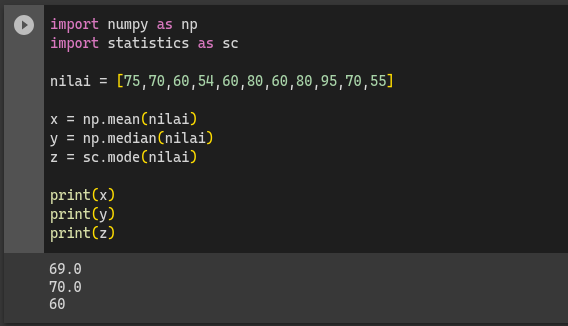
\includegraphics[height=4cm]{./images/q3.png}
\end{center}

\begin{align*}
    \text{Data} = [75, 70, 60, 54, 60, 80, 60, 80, 95, 70, 55]\\
    \text{Sorted} = [54, 55, 60, 60, 60, 70, 70, 75, 80, 80, 95]
\end{align*}

\begin{itemize}
    \item {
        \textbf{Mean}:

        \begin{align*}
            \bar{x} &= \frac{\sum_ x}{n} \\
            &= \frac{75 + 70 + 60 + 54 + 60 + 80 + 60 + 80 + 95 + 70 + 55}{11} \\
            &= \frac{759}{11} \\
            &= 69
        \end{align*}
    }
    \item {
        \textbf{Median}:
        Since the data is ungrouped and the count is odd, the median is the middle value, which is 70.
    }
    \item {
        \textbf{Mode}:
        Since the data isn't grouped, we can find the most occuring value which is 60.
    }
\end{itemize}

\pagebreak

\subsection{Question 4}
Find the mode from this data

\begin{center}
    \begin{tabular}{|c|c|}
        \hline
        Value & Frequency \\
        \hline
        5 - 10 & 4 \\
        \hline
        11 - 16 & 6 \\
        \hline
        17 - 22 & 12 \\
        \hline
        23 - 28 & 8 \\
        \hline
        29 - 34 & 8 \\
        \hline
    \end{tabular}
\end{center}

\textbf{Mode}:

\begin{align*}
    \text{Mode} &= \text{L} + \text{c} \left( \frac{l}{l+u} \right) \\
    &= 16.5 + 5 \left( \frac{(12-8)}{(12-8) + (12-6)} \right) \\
    &= 16.5 + 5 \left( \frac{4}{4 + 6} \right) \\
    &= 16.5 + 5 \left( \frac{4}{10} \right) \\
    &= 16.5 + 2 \\
    &= 18.5
\end{align*}

\pagebreak

\subsection{Question 5}
Determine the mean and median

\begin{center}
    \begin{tabular}{|c|c|}
        \hline
        Value & Frequency \\
        \hline
        11 - 20 & 3 \\
        \hline
        21 - 30 & 5 \\
        \hline
        31 - 40 & 10 \\
        \hline
        41 - 50 & 11 \\
        \hline
        51 - 60 & 8 \\
        \hline
        61 - 70 & 3 \\
        \hline
    \end{tabular}
\end{center}

\begin{itemize}
    \item {
        \textbf{Mean}:

        \begin{align*}
            \bar{x} &= \frac{\sum x_i f_i}{n}\\
            &= \frac{(15)(3) + (25)(5) + (35)(10) + (45)(11) + (55)(8) + (65)(3)}{40} \\
            &= \frac{45 + 125 + 350 + 495 + 440 + 195}{40} \\
            &= \frac{1650}{40} \\
            &= 41.25
        \end{align*}
    }
    \item {
        \textbf{Median}:

        \begin{align*}
            \text{Me} &= b + p \left( \frac{\frac{1}{2}n - F}{f} \right)\\
            &= 40.5 + 10 \left( \frac{\frac{1}{2}(40) - 10}{11} \right) \\
            &= 40.5 + 10 \left( \frac{20 - 10}{11} \right) \\
            &= 40.5 + 10 \left( \frac{10}{11} \right) \\
            &= 40.5 + 9.09 \\
            &= 49.59
        \end{align*}
    }
\end{itemize}

Corrector: Yanuar Thaif Chalil Candra

Value: 57


\end{document}
